%\part*{Lezione 10/03/2021}
\paragraph{Sui risultati della first order perturbation theory} 
Possiamo rielaborare le espressioni per $E_{JM}$ e $M_{JM}$ sostituendo\footnote{In realtà quello che facciamo è integrare per parti e poi usare il teorema di Gauss.} i termini di corrente che abbiamo calcolato:
\begin{displaymath}
\begin{aligned}
E_{JM}(k) &= \frac{1}{k} \int d^3x \; \Bigl \{ [\vec{\nabla}\land \mathrm{j}_J(kx) \vec{\mathcal{Y}}^M_{JJ1}] \cdot \vec{J}_C(\vec{x}) + k^2 \mathrm{j}_J(kx) \:\vec{\mu}(\vec{x})\cdot\vec{\mathcal{Y}}^M_{JJ1} \Bigr \} \\
M_{JM}(k) &=  \int d^3x \; \Bigl \{ \mathrm{j}_J(kx) \vec{\mathcal{Y}}^M_{JJ1}\cdot \vec{J}_C(\vec{x}) + \:\vec{\mu}(\vec{x})\cdot[\vec{\nabla}\land \mathrm{j}_J(kx) \vec{\mathcal{Y}}^M_{JJ1}] \Bigr \}
\end{aligned}
\end{displaymath}
Se $k\ll 1$ (situazione frequente) allora sarà dominante in $E$ il termine di corrente $\vec{J}_C$; inoltre a parità di $J$ per $k$ piccolo abbiamo $\mathrm{j}_J\sim (kx)^J$ per cui $E_{JM}>M_{JM}$ (come avevamo trovato per le stime di Weisskopf\index{stime di Weisskopf}).

\paragraph{Stima del dipolo} Riprendiamo l'espressione dell'hamiltoniana di interazione\footnote{Da qui in poi chiameremo il versore di polarizzazione $\widehat{\varepsilon}$ con $\hat{e}$ per semplicità di scrittura.}:
$$\int d^3x \; e^{-i\vec{k}\cdot\vec{x}}\widehat{\varepsilon}^*_{\vec{k}\lambda}\cdot\vec{J} (\vec{x})$$
Poiché $k< 1$ MeV$/\hbar c$ (spesso si prende dell'ordine del keV) si ha che\footnote{Si tratta della stessa approssimazione fatta per il decadimento $\beta$ e nasce dal fatto che il decadimento si osserva soprattutto nel caso di nuclei pesanti.} $\mean{\vec{k}\cdot\vec{x}_i}\simeq 10/200 = 1/20\ll 1$, quindi è ragionevole assumere la \textbf{Long Wavelength Approximation}\index{long wavelength approximation}. Nel calcolo dell'elemento di matrice, sfruttando la $\delta^3(\vec{x}-\vec{x}_i)$ che compare nell'espressione della corrente possiamo riscrivere l'esponenziale come $\exp{(i\vec{k}\cdot\vec{x}_i)}$ e quindi approssimarlo $\sim 1$, per cui:
$$\int d^3x\; \hat{e}_{k\lambda}^* \cdot \vec{J}(\vec{x}) = \int d^3x\; \hat{e}_{k\lambda}^* \cdot (\vec{J}(\vec{x})\cdot \vec{\nabla})\,\vec{x} = - \int d^3x \; \hat{e}_{k\lambda}^* \cdot \vec{x}\, (\vec{\nabla}\cdot\vec{J}(\vec{x})) $$
dove abbiamo usato $\Div{x} = \partial_j \,i = \delta_{ji}$ e abbiamo integrato per parti. Dall'equazione di continuità (valutata sugli stati iniziale e finale) si ha $\mean{\vec{\nabla}\cdot\vec{J}(\vec{x})} = -i\mean{[H,\rho]} = -i(E_f-E_i)\mean{\rho} = i E_\gamma \mean{\rho}$, quindi possiamo riscrivere:
$$\oss{J_fM_f}{\int d^3x \; \hat{e}^*_{k\lambda}\cdot \vec{J}(\vec{x})}{J_iM_i} = -iE_\gamma \, \oss{J_fM_f}{\int d^3x \; \hat{e}^*_{k\lambda}\cdot \vec{x}\rho}{J_iM_i} = -i E_\gamma \, \hat{e}^*_{k\lambda} \cdot \vec{\mathrm{d}}_{fi}$$
$$\vec{\mathrm{d}}_{fi} \equiv \oss{J_fM_f}{\int d^3x \; \vec{x}\rho}{J_iM_i}$$
dove $\vec{\mathrm{d}}_{fi}$ è l'\textbf{operatore di dipolo elettrico}\index{operatore di dipolo elettrico}.\\
Generalizzando per ogni termine di multipolo\footnote{Trascuriamo il secondo termine di $E_{JM}$ perché stiamo considerando $k$ piccoli.}:\index{termini di multipolo!elettrico}\index{termini di multipolo!magnetico}
\begin{displaymath}
\begin{aligned}
E_{JM} &\simeq \frac{k^J}{(2J+1)!!} \sqrt{\frac{J+1}{J}}\, \int d^3x \; \Bigl [ x^J \mathcal{Y}_{JM}(\hat{x})\rho(\vec{x}) \Bigr ] \\
M_{JM} &\simeq i\frac{k^J}{(2J+1)!!} \sqrt{\frac{J+1}{J}}\, \int d^3x \; \Bigl [ \vec{\mu}(\vec{x}) + \frac{1}{J+1} \vec{r}\land \vec{J}_C(\vec{x}) \Bigr ]\cdot \vec{\nabla}\,x^J\mathcal{Y}_{JM}(\hat{x})
\end{aligned}
\end{displaymath}
In realtà, non è necessario calcolarli esplicitamente per ogni $M$, perché questi (che indichiamo con $T_{JM}$ dove $T=E,M$) sono operatori irriducibili e di conseguenza applicando il teorema di Wigner-Eckart\index{teorema di Wigner-Eckart} si ha:
$$\oss{J_fM_f}{T_{JM}}{J_iM_i} = \underbrace{\frac{(-)^{J_i-M_i}}{\sqrt{2J+1}}\clebs{J_fM_f,\,J_i\, -M_i}{J,M}}_{\text{Dipendenza da }M}\; \underbrace{\bigl\langle\, J_f\, ||\,T_J\, ||\,J_i\, \bigr\rangle}_\text{Elemento di matrice ridotta}$$
Nell'espressione della sezione d'urto è l'elemento di matrice ridotta\index{elemento di matrice ridotta} che compare e dunque può essere calcolato scegliendo il valore di $M$ per il quale è più semplice valutare $\oss{J_fM_f}{T_{JM}}{J_iM_i}$.

\subparagraph{Probabilità di decadimento per il dipolo} Procediamo con il calcolo\footnote{Nei calcoli tenderemo a tenere $c=\hbar=1$.} della probabilità di decadimento per il dipolo elettrico (ci aspettiamo di ritrovare il risultato classico).\\
Facciamo l'ipotesi di \textit{long wavelength approximation}\index{long wavelength approximation}, per cui\footnote{In questo caso chiamiamo l'elemento di matrice di transizione con $T_{fi}$.}:
$$d\lambda = \sum_{k\lambda} \frac{2\pi}{\hbar} \delta(E_i-E_f-E_\gamma) \,|T_{fi}|^2 \:\Omega \frac{d^3k}{(2\pi)^3}$$
$$T_{fi}\equiv -\frac{e}{\sqrt{2\omega_k \Omega}}\,i E_\gamma \, \hat{e}^*_{k\lambda}\cdot \vec{\mathrm{d}}_{fi}$$
dove la somma su $\vec{k}$ è intesa sullo spazio delle fasi e  $\omega_k = E_\gamma$.
\begin{figure}[h]
    \centering
    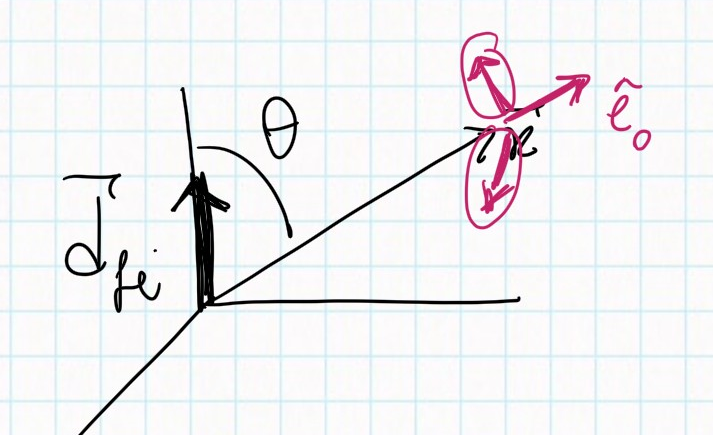
\includegraphics[scale=0.2]{Immagini/0310_sistema.png}
    \caption{Rappresentazione del sistema in esame.}
    \label{0310_sist}
\end{figure}
\newline
\noindent Soffermiamoci sull'elemento di matrice $|\hat{e}^*_{k\lambda}\cdot \vec{\mathrm{d}}_{fi}|^2$, facendo riferimento allo schema in Figura \ref{0310_sist}.
$$\sum_{\lambda = \pm 1}|\hat{e}^*_{k\lambda}\cdot \vec{\mathrm{d}}_{fi}|^2 = \sum_{\lambda=-1}^{+1} |\hat{e}^*_{k\lambda}\cdot \vec{\mathrm{d}}_{fi}|^2 - |\hat{e}^*_{k0}\cdot \vec{\mathrm{d}}_{fi}|^2 = \mathrm{d}_{fi}^2 -\mathrm{d}_{fi}^2\cos^2{(\theta)} = \mathrm{d}_{fi}^2 \sin^2{(\theta)} $$
Allora avremo per il rate:
\begin{displaymath}
\begin{aligned}
d\lambda &= \frac{2\pi}{\hbar} \delta(E_i-E_f-E_\gamma) \,\frac{e^2}{2}E_\gamma \mathrm{d}_{fi}^2 \sin^2(\theta) \,  \frac{k^2dkd\hat{k}}{(2\pi)^3} \\
%
p_\gamma = \hbar k \;\; E_\gamma = p_\gamma c &\qquad\frac{p^2_\gamma dp_\gamma}{\hbar^3} \to \frac{E_\gamma^2 dE_\gamma}{(\hbar c)^3}\\
%
\frac{d\lambda}{d\hat{k}} &= \frac{2\pi}{\hbar} \delta(E_i-E_f-E_\gamma) \,\frac{e^2}{2}E_\gamma \mathrm{d}_{fi}^2 \sin^2(\theta) \, \frac{E_\gamma^2 dE_\gamma}{(2\pi\hbar c)^3} \\
%
\Rightarrow \; \frac{d\lambda}{d\hat{k}} &= \frac{2\pi}{\hbar} \,\frac{e^2}{2}E_\gamma^3 \, \frac{\mathrm{d}_{fi}^2 \sin^2(\theta)}{(2\pi \hbar c)^3} \\
%
\frac{d\lambda}{d\hat{k}} &= \frac{1}{\hbar} \frac{\alpha}{2\pi}\,E_\gamma^3 \, \frac{\mathrm{d}_{fi}^2 \sin^2(\theta)}{( \hbar c)^2}
\end{aligned}
\end{displaymath}
dove nel penultimo passaggio abbiamo integrato la $\delta$ per cui $E_\gamma = E_i - E_f$ e nell'ultimo abbiamo sostituito la costante di struttura fine\index{costante di struttura fine@$\alpha$-costante di struttura fine} $\alpha$. Possiamo notare che abbiamo ottenuto un andamento del tipo $E^3_\gamma \sin^2(\theta)$ come nel caso classico.

\subsection{Riassunto}
Riassumiamo i concetti base del decadimento $\gamma$ che abbiamo sviluppato finora.
\begin{itemize}
    \item Fissato $J$, i termini di multipolo elettrico e magnetico hanno parità opposta.
    \item A parità di $J$ il contributo elettrico è maggiore rispetto a quello magnetico.
\end{itemize}

\subsubsection{Regole di selezione}
Poiché $\vec{J}_i = \vec{J}_f + \vec{J}$, si ha che $|J_i - J_f|\leq J\leq J_i+J_f$ e $\pi_i = \pi_f \cdot \pi(T_J)$, da cui derivano di conseguenza delle regole di selezione per i vari termini (non tutti i multipoli sono ammessi):
\begin{itemize}
    \item Se $\pi_i = \pi_f$: allora per $M$ ho $J$ dispari e per $E$ ho $J$ pari.
    \item Se $\pi_i \not = \pi_f$: allora per $E$ ho $J$ dispari e per $M$ ho $J$ pari.
\end{itemize}
Notiamo che $J > 0$ anche se $J_i=J_f$, infatti se così non fosse (ovvero $J=0$) allora avremmo un fotone emesso lungo $\hat{k}$, ma questo non è possibile (solo polarizzazione $\pm 1$). Dunque le transizioni $0\to 0$ non sono ammesse\footnote{Queste si vedono, ma sono dovute a un processo differente, ovvero avvengono per \textbf{conversione interna}: il nucleo interagisce con un elettrone dell'atomo e quest'ultimo viene emesso.}.

\subsection{Alcuni esempi}
\paragraph{Primo esempio}
$$\ce{^{60}Co}  \xrightarrow{\beta^-} \ce{^{60}Ni}^*  \xrightarrow{\gamma}  \ce{^{60}Ni}$$

\begin{figure}[h]
    \centering
    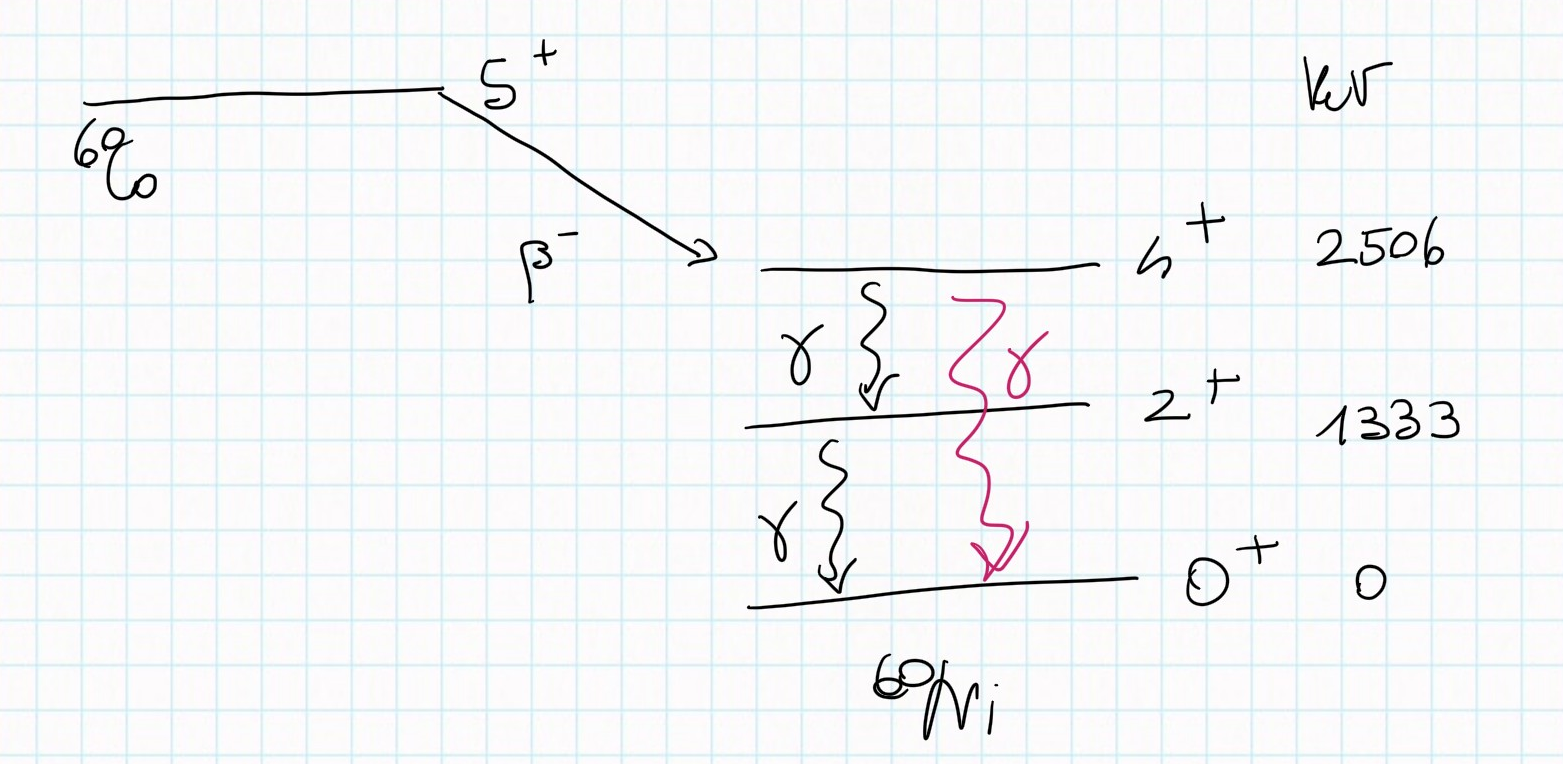
\includegraphics[scale=0.2]{Immagini/0310_bande.png}
    \caption{Schema delle bande rotazionali\index{bande rotazionali} coinvolte nel decadimento.}
    \label{0310_bande}
\end{figure}

\noindent Come mostrato nello schema in Figura \ref{0310_bande}, abbiamo 3 possibilità di decadimento:
\begin{itemize}
    \item $4^+\to2^+$: in questo caso $2\leq J\leq 6$ e $\delta \pi = 0$, allora avremo $E2,\,M3,\,E4,\,M5,\,E6$, dove domina per $E_\gamma\simeq 1.2$ MeV ($k\ll 1$) solo $E2$, con $M3$ come correzione.
    \item $2^+\to0^+$: in questo caso $J=2$ e $\delta \pi = 0$, allora avremo $E2$.
    \item $4^+\to0^+$: in questo caso $J=4$ e $\delta \pi = 0$, allora avremo $E4$.
\end{itemize}
\noindent  Per quanto riguarda le stime di Weisskopf\index{stime di Weisskopf}, ovviamente non saranno precise perché queste sono bande rotazionali\index{bande rotazionali}, quindi non è possibile fare l'approssimazione di simmetria sferica; tuttavia permettono di ottenere l'ordine di grandezza:
\begin{displaymath}
\begin{aligned}
\lambda(E2) &\simeq 7\cdot 10^7 \, 60^{4/3}\, (1.2)^5 \sim 2\cdot 10^{10} \unit{s}^{-1} & \tau_{dec} &= \frac{1}{\lambda} \sim 10^{-10} \unit{s} & 4^+&\to2^+ \\
%
\lambda(E2) &\simeq 7\cdot 10^7 \, 60^{4/3}\, (1.3)^5 \sim 2\cdot 10^{10} \unit{s}^{-1} & \tau_{dec} &= \frac{1}{\lambda} \sim 10^{-10} \unit{s} & 2^+&\to0^+ \\
%
\lambda(E4) &\simeq 10^{-5} \, 60^{8/3}\, (2.5)^5 \sim 2 \unit{s}^{-1} & \tau_{dec} &= \frac{1}{\lambda} \sim 0.5 \unit{s} & 4^+&\to0^+ 
\end{aligned}
\end{displaymath}
dove si può notare che tra $E2$ ed $E4$ c'è un fattore $10^{10}$. 

\paragraph{Secondo esempio}
$$\ce{^{137}Cs}  \xrightarrow{\beta^-} \ce{^{137}Ba}^*  \xrightarrow{\gamma}  \ce{^{137}Ba}$$

\begin{figure}[h]
    \centering
    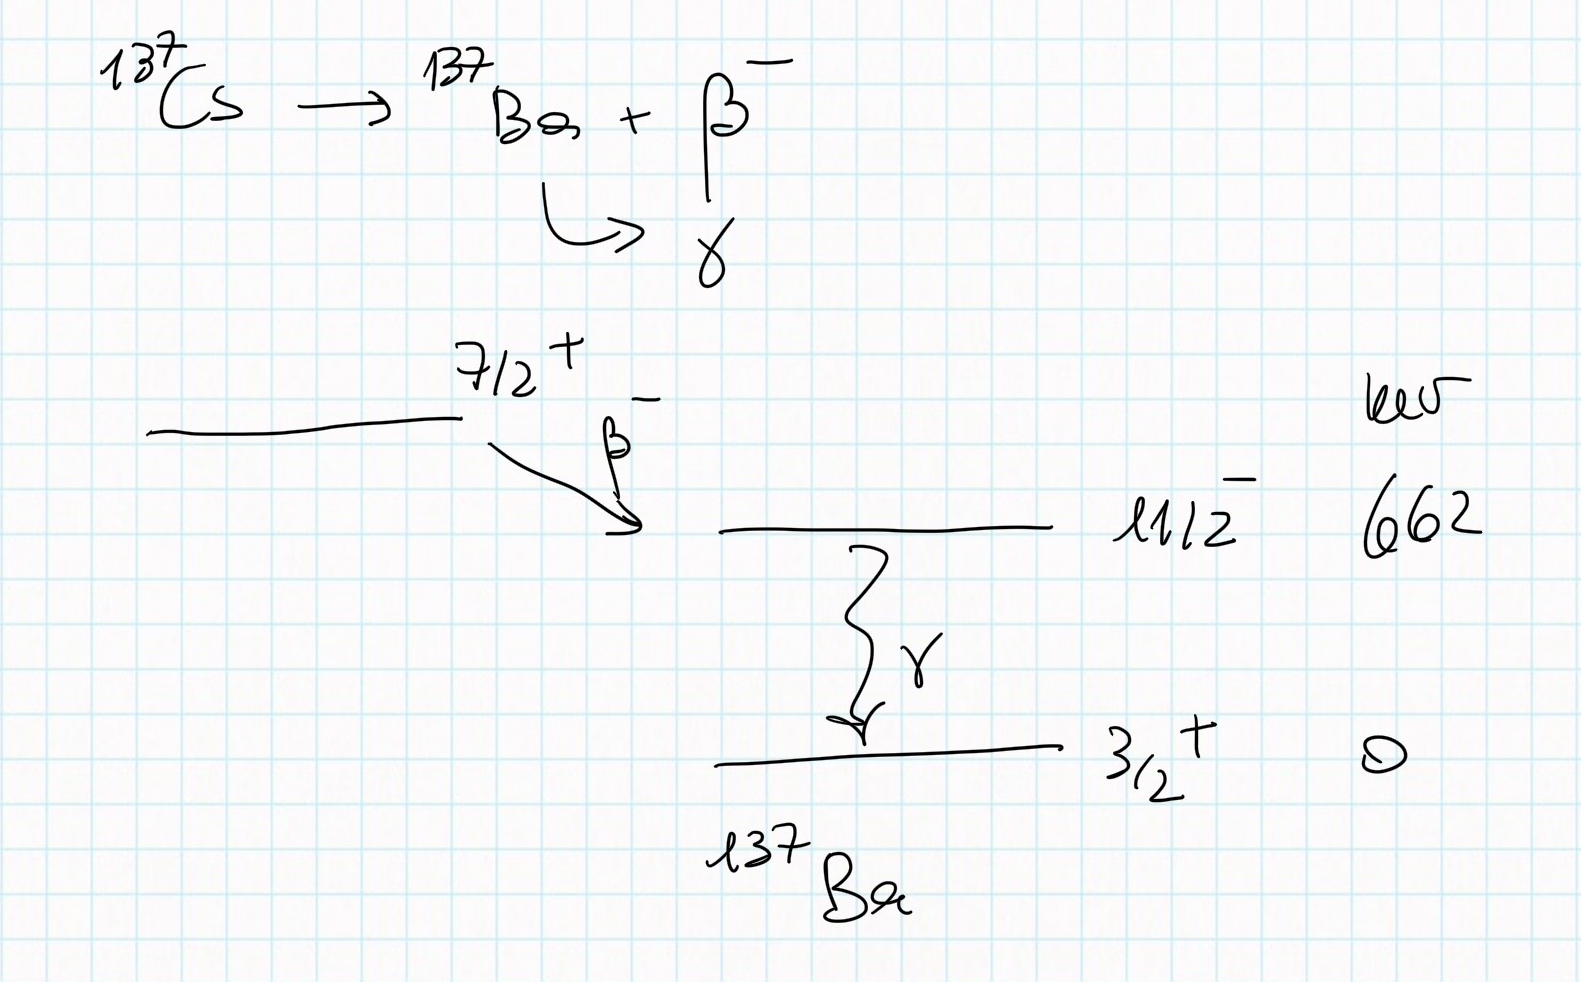
\includegraphics[scale=0.2]{Immagini/0310_bande2.png}
    \caption{Schema delle bande rotazionali\index{bande rotazionali} coinvolte nel decadimento.}
    \label{0310_bande1}
\end{figure}

\noindent In questo caso abbiamo la transizione $\frac{11}{2}^-\to\frac{3}{2}^+$ per cui $4\leq J \leq 7$ e $\Delta\pi \not = 0$; allora i termini di multipolo saranno $M4,\,E5,\,M6,\,E7$, dove $M4$ sarà dominante e $E5$ una piccola correzione.


\paragraph{Terzo esempio}
$$\ce{^{176}_{71}Lu}  \xrightarrow{\beta^-} \ce{^{176}_{72}Hf}^*  \xrightarrow{\gamma}  \ce{^{176}_{72}Hf}$$

\begin{figure}[h]
    \centering
    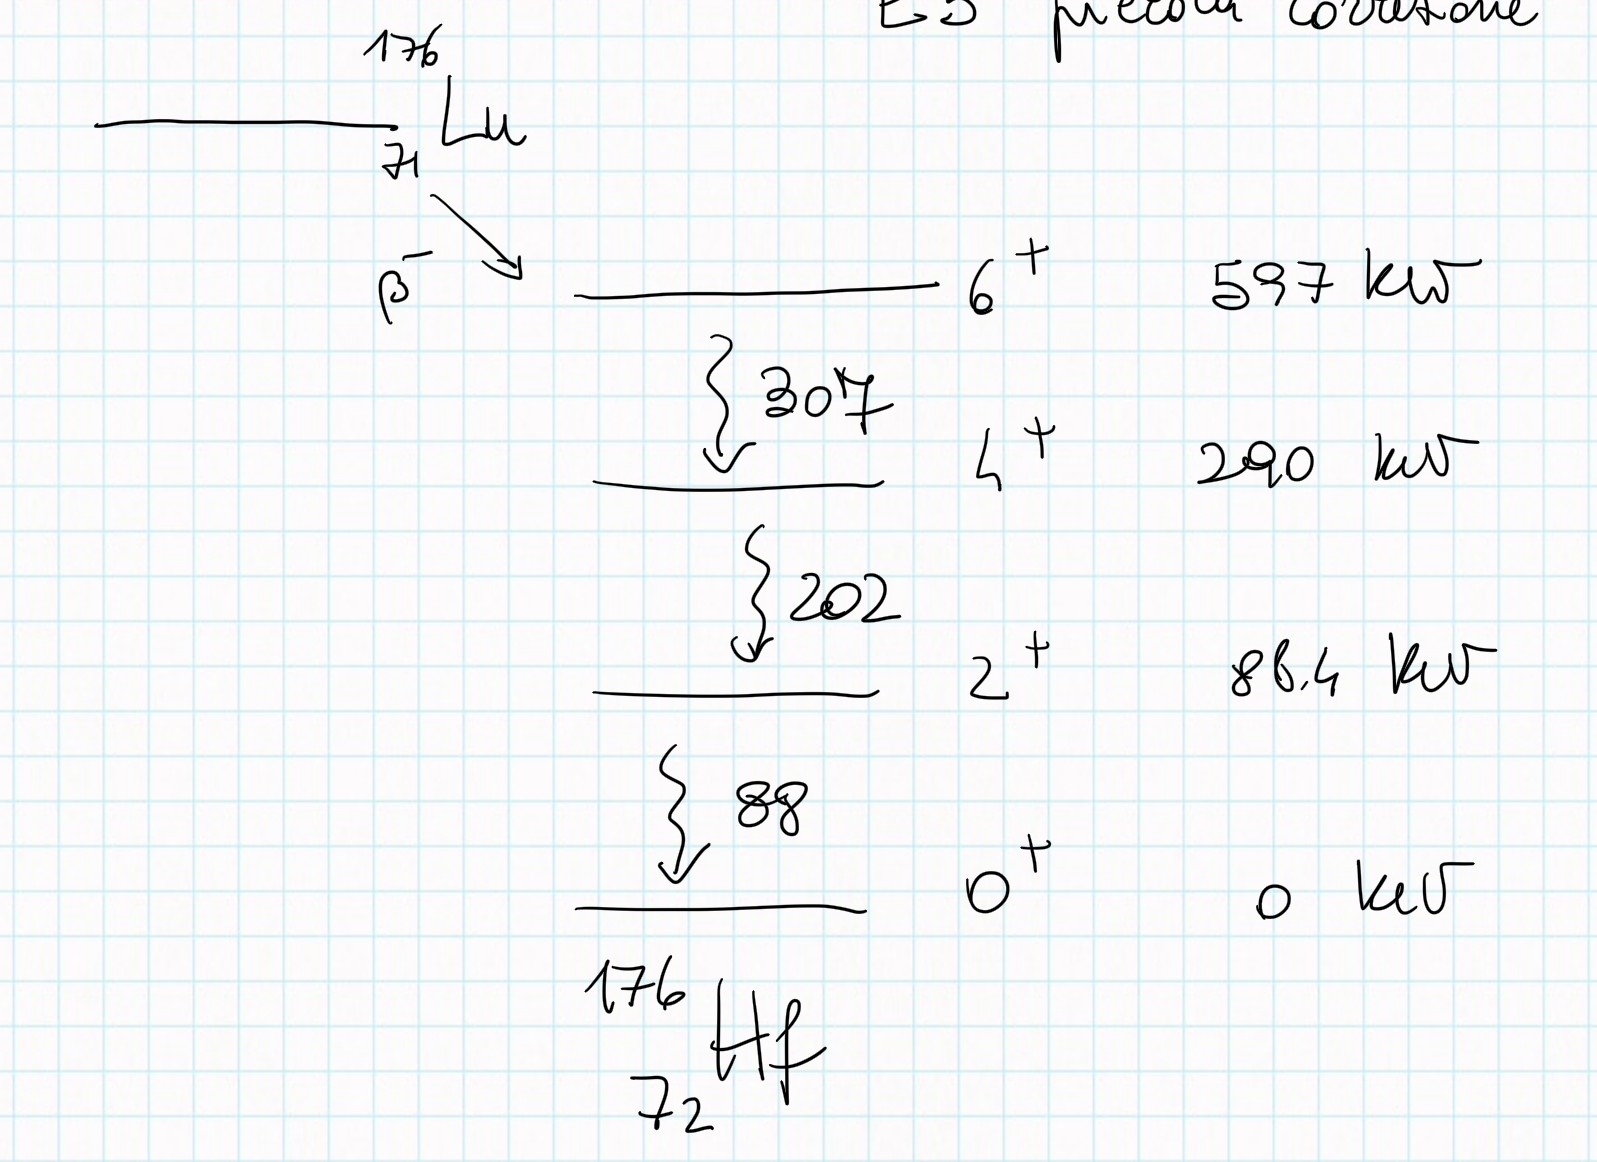
\includegraphics[scale=0.2]{Immagini/0310_bande3.png}
    \caption{Schema delle bande rotazionali\index{bande rotazionali} coinvolte nel decadimento.}
    \label{0310_bande2}
\end{figure}

\noindent In tutti i casi $\Delta\pi =0 $, studiamo $J$:
\begin{enumerate}[1.]
    \item $6^+\to4^+$: abbiamo $2\leq J \leq 10$, dominante $E2$.
    \item $4^+\to2^+$: abbiamo $2\leq J \leq 6$, dominante $E2$.
    \item $2^+\to0^+$: abbiamo $J=2$, dominante $E2$.
\end{enumerate}
Guardiamo le stime di Weisskopf\index{stime di Weisskopf}:
\begin{displaymath}
\begin{aligned}
1& & E2&\simeq 1.9 \cdot 10^8 \unit{s}^{-1} & \tau_{\frac{1}{2}} \simeq 3.6 \cdot 10^{-9} \unit{s} \\
2& & E2&\simeq 2.4 \cdot 10^7 \unit{s}^{-1} & \tau_{\frac{1}{2}} \simeq 2.9 \cdot 10^{-8} \unit{s} \\
3& & E2&\simeq 3.8 \cdot 10^5 \unit{s}^{-1} & \tau_{\frac{1}{2}} \simeq 1.8 \cdot 10^{-6} \unit{s} 
\end{aligned}
\end{displaymath}
Poiché i decadimenti 1 e 2 sono molto più veloci del decadimento 3 li osserverò come fondo di quest'ultimo (in un esperimento che ha come interesse lo studio del decadimento 3). Tuttavia, il risultato sperimentale del decadimento 3 $\tau_{\frac{1}{2}}^{oss}\simeq 1.43\cdot10^{-9}$ s non è assolutamente compatibile con quanto atteso; ciò è dovuto principalmente al fatto della asimmetria del nucleo, come già avevamo accennato: le stime di Weisskopf\index{stime di Weisskopf} non sono precise per nuclei particolarmente deformati (come in questo caso).

\subsection{Stato di scattering}
Vogliamo in questa trattazione studiare $J$, quindi non ci interessa che le particelle coinvolte siano nuclei o meno. Prendiamo lo stato di scattering:
$$n+p \to d + \gamma$$
Possiamo sempre definire lo stato iniziale come un autostato del momento $J$ ed espanderlo in onde parziali $\psi_{np}$. Allora avremo $\ell = 0,1,2,\dots$, ma dal momento che lo stato è di scattering (basse energie) ci interessa solo $\ell=0$; per quanto riguarda lo spin avremo $S=0,1$, tuttavia poiché i coefficienti di Clebsch-Gordan\index{coefficienti di Clebsch-Gordan} della transizione ${^3S_1}\to {^3S_1}$ sono trascurabili rispetto a quelli della transizione ${^1S_0}\to {^3S_1}$ avremo che rimarrà\footnote{Il pezzo di corrente di magnetizzazione in questo caso è rilevante ($k\to0$).} solo $S=0$.\\
Dunque, abbiamo ${^1S_0}\to {^3S_1}$ con $J=1$ e $\Delta\pi  = 0$ e il termine dominante sarà $M1$.\\
Tuttavia, approfondiremo questo studio nella sezione \secrif{0317-sec-abinitio}.
